\section{Data Quality Checks}

This section documents the basic data quality checks for ALEPH archieved data collected in the LEP1 and LEP2 period. In additional to the raw spectra from the data, jet and particle spectra are compared to the predictions from PYTHIA8 event generator (Version 8.230 Default Tune). 

\subsection{LEP1 vs LEP1 Monte-Carlo}
\begin{figure}[H]
\centering
\subfloat{\label{sfig:a}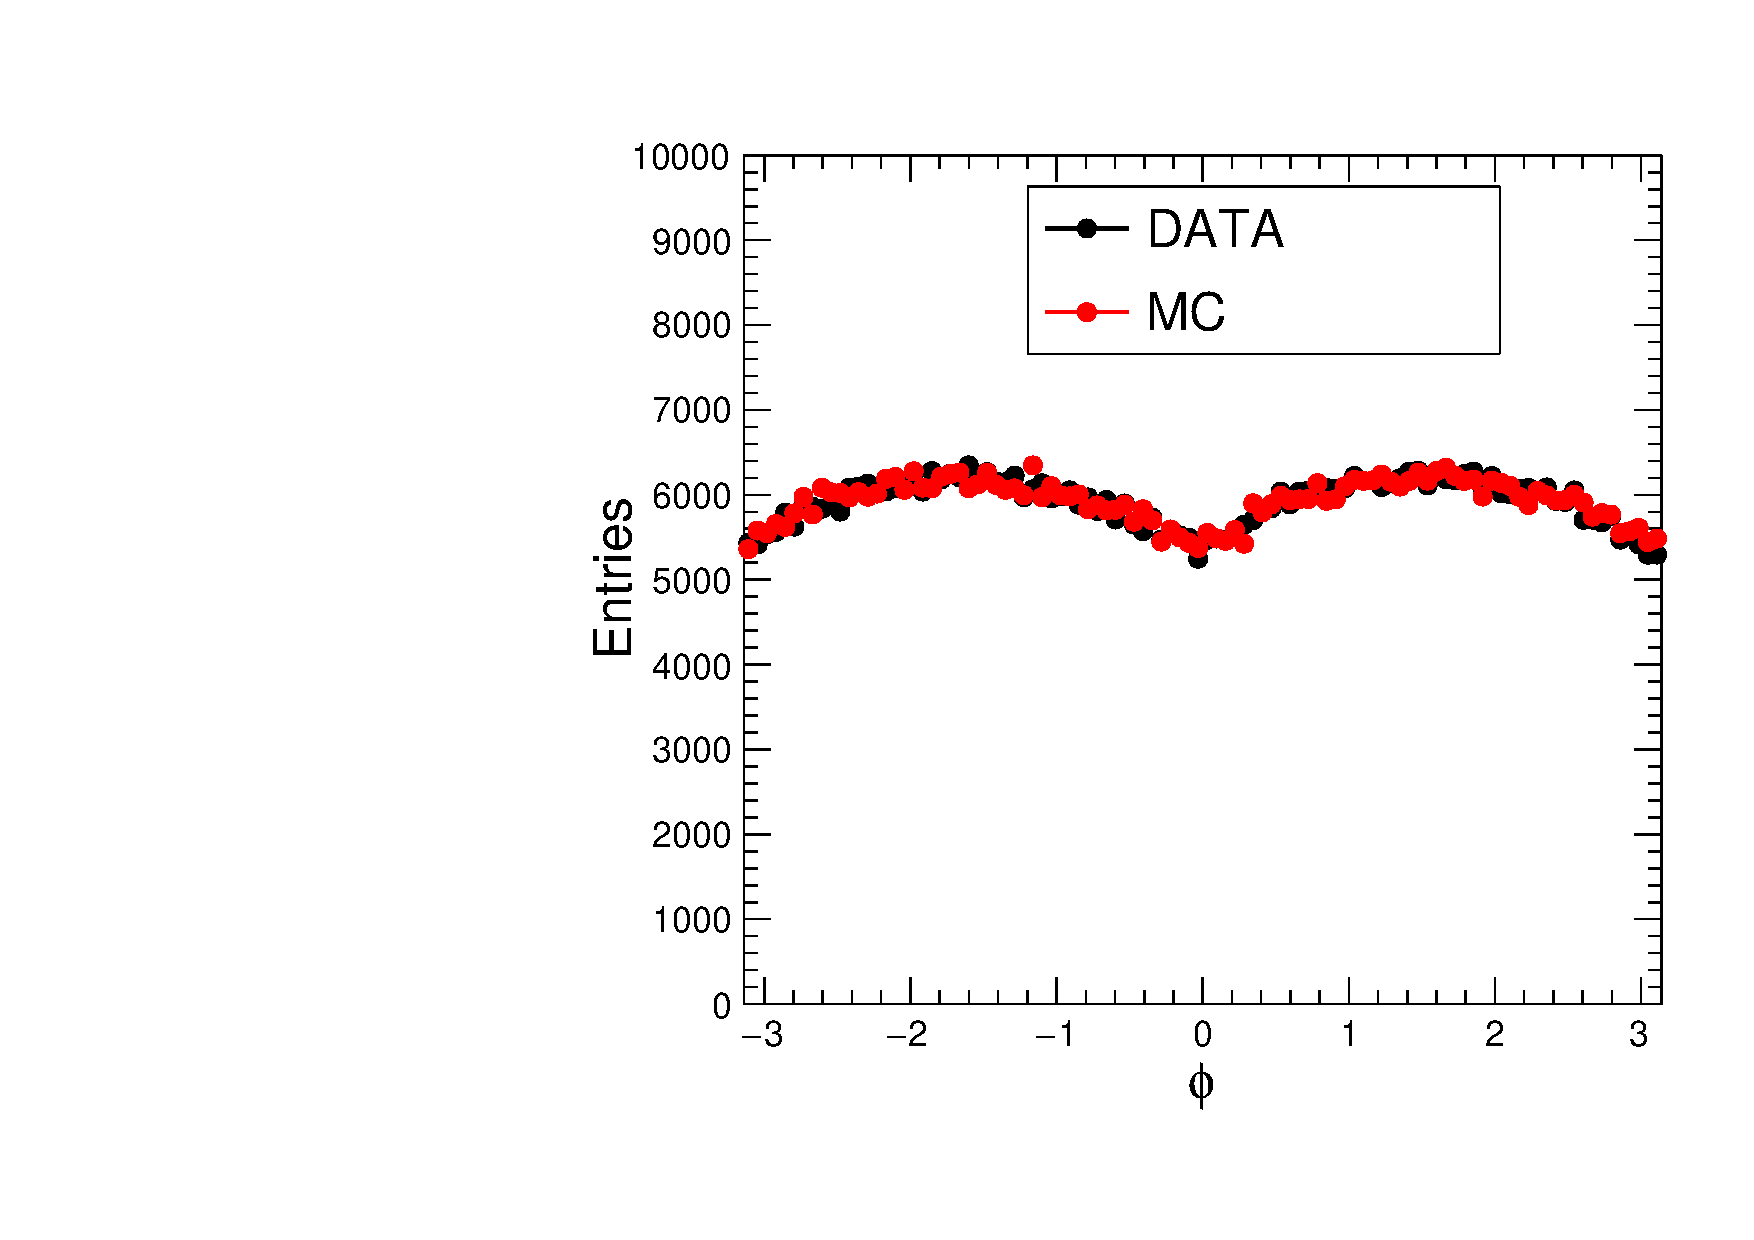
\includegraphics[width=.30\textwidth]{images/datamc/canvasPhiPreES.pdf}}\hfill
\subfloat{\label{sfig:b}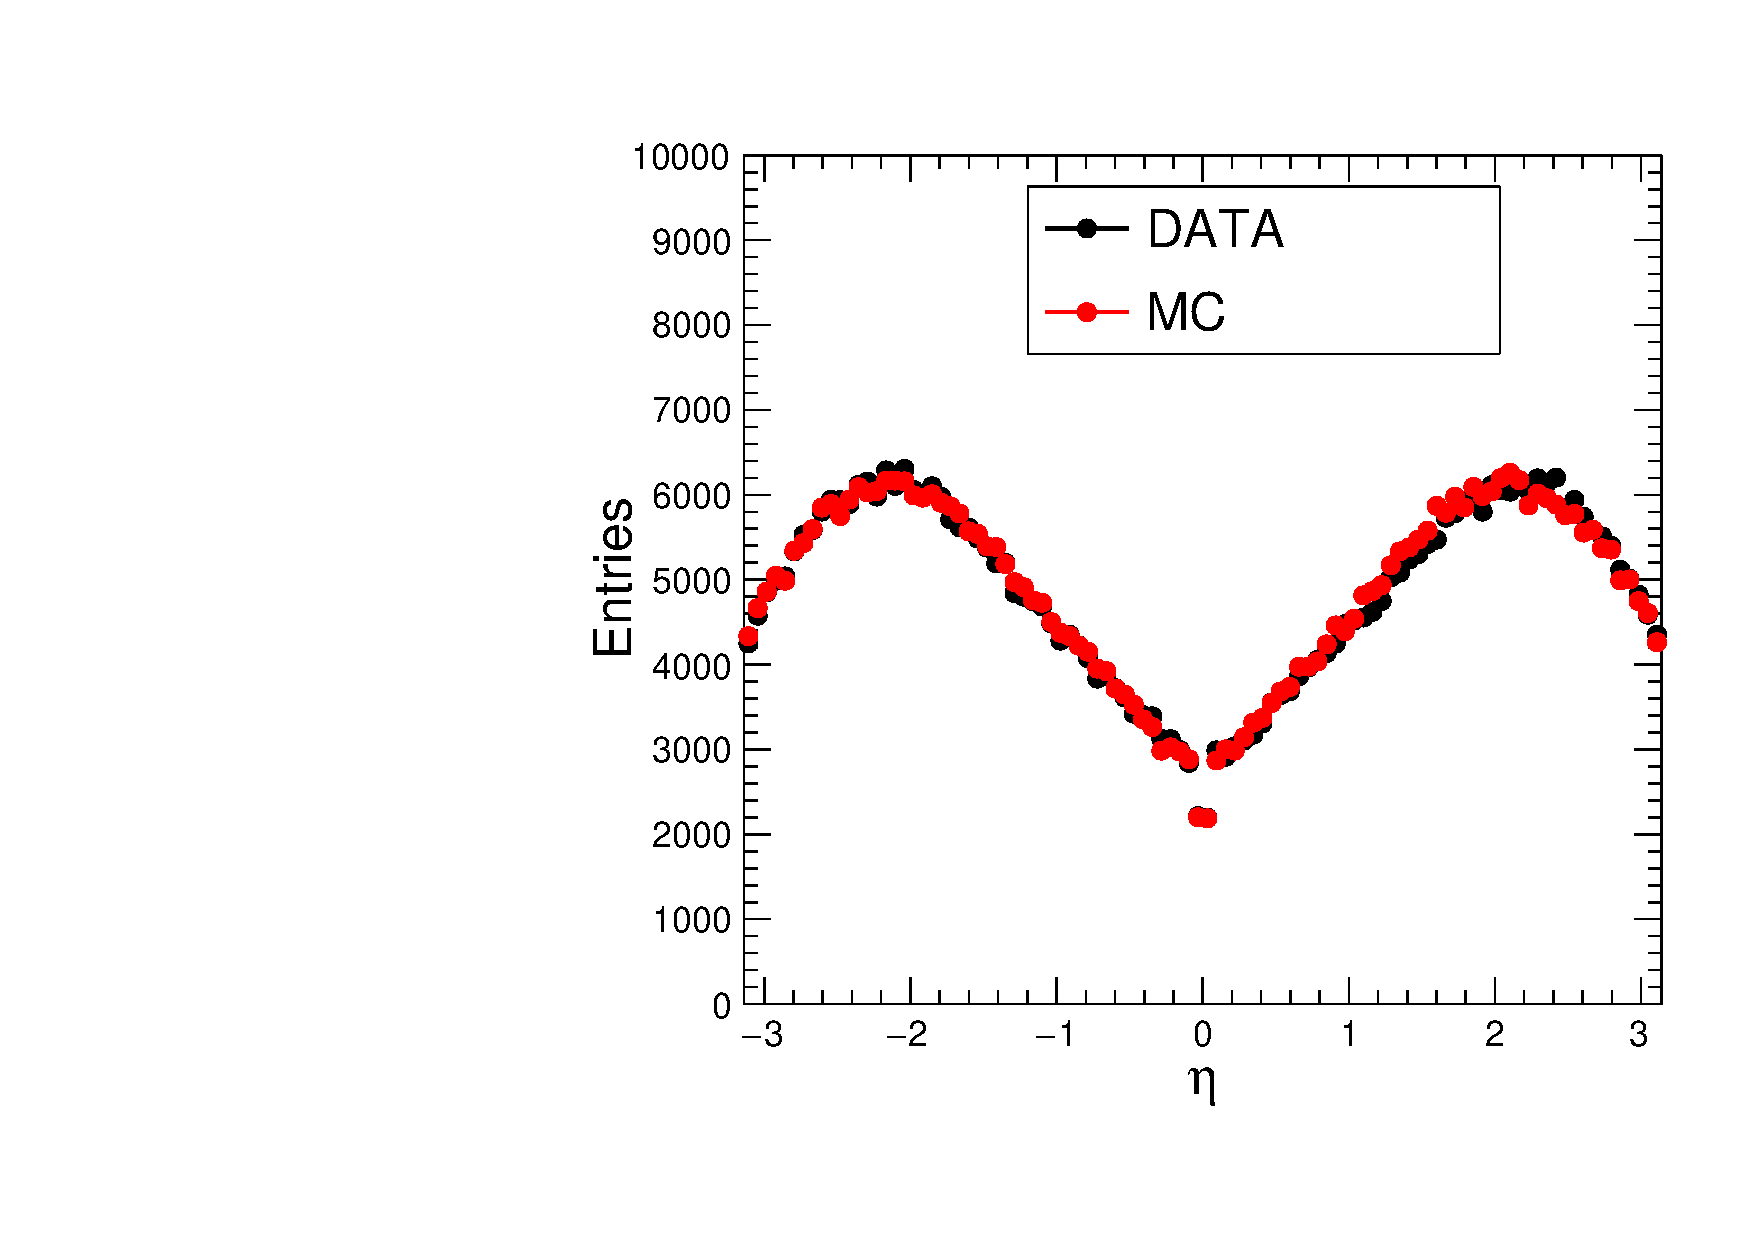
\includegraphics[width=.30\textwidth]{images/datamc/canvasetaPreES.pdf}}\hfill
\subfloat{\label{sfig:c}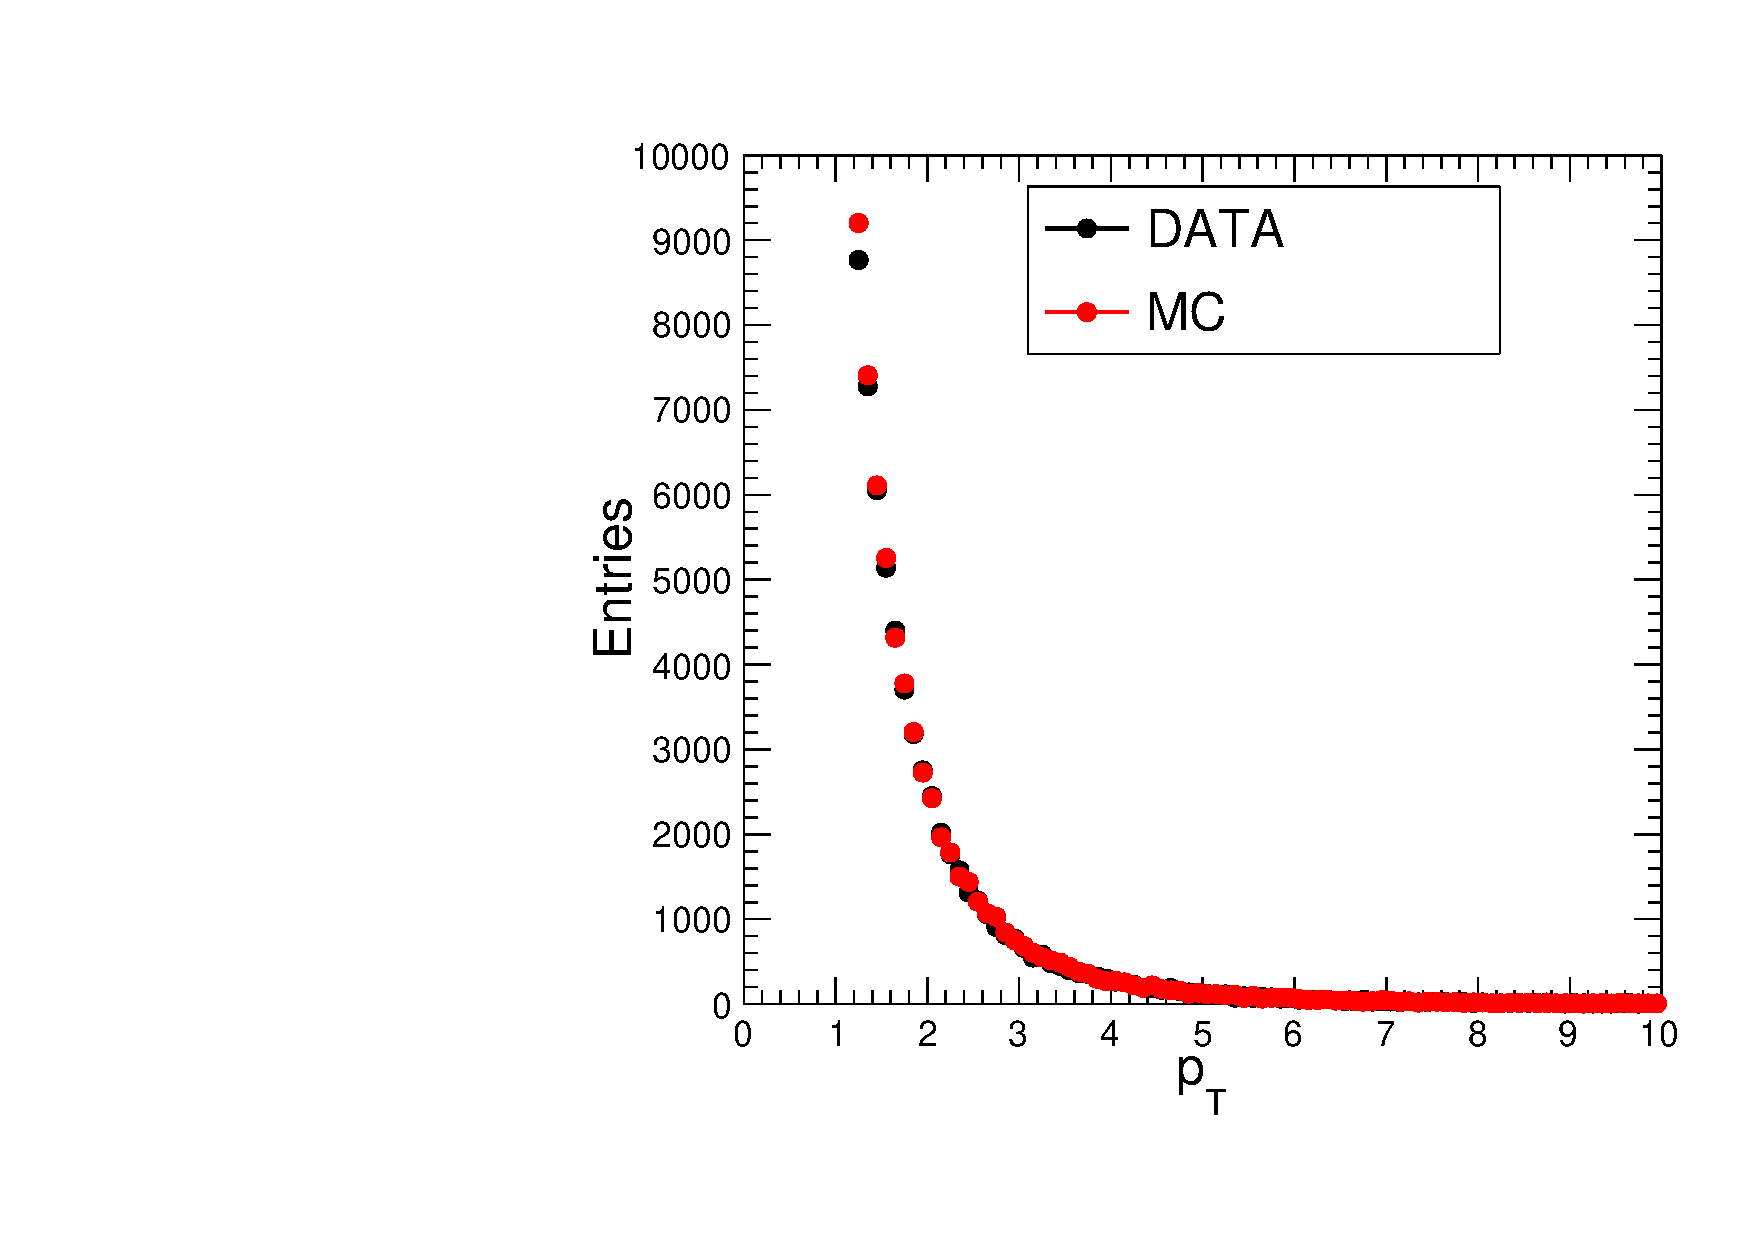
\includegraphics[width=.30\textwidth]{images/datamc/canvasptPreES.pdf}}\hfill
\caption{}  
\end{figure}

\iffalse
\subsection{LEP1 Track Efficiency}
\begin{figure}[H]
\centering
\subfloat{\label{sfig:a}\includegraphics[width=.30\textwidth]{images/trkefficiency/ptclean.pdf}}\hfill
\subfloat{\label{sfig:b}\includegraphics[width=.30\textwidth]{images/trkefficiency/thetaclean.pdf}}\hfill
\subfloat{\label{sfig:c}\includegraphics[width=.30\textwidth]{images/trkefficiency/phiclean.pdf}}\hfill
\caption{Track efficiency for LEP1 data. Cuts used in each plot are listed in the title.}
\end{figure}

\begin{figure}[H]
\centering
\subfloat{\label{sfig:a}\includegraphics[width=.30\textwidth]{images/trkefficiency/ptratio.pdf}}\hfill
\subfloat{\label{sfig:b}\includegraphics[width=.30\textwidth]{images/trkefficiency/thetaratio.pdf}}\hfill
\subfloat{\label{sfig:c}\includegraphics[width=.30\textwidth]{images/trkefficiency/phiratio.pdf}}\hfill
\caption{Track efficiency closure tests for LEP1 data.}
\end{figure}

\fi
